\section{Scattering}

Consider an electric charge $+q$ which stricken by an incident electromagnetic
field with a certain frequency $\omega$. An electromagnetic force is then exerted
on the charge which accelerates it. Consequently, the electric charge will emit
radiation.

\subsection{Thomson scattering}

Consider a free charge $q$ in its restframe $\vec{v} = 0$ (or $v \approx 0$)
striken by an electromagnetic field $\vec{E} = \hat{e} E \cos
\klammer{\omega t - \vec{k} \cdot \vec{x}}$. The force acting on the charge,
placed at $\vec{x} =0$ is:
\begin{align*}
    \vec{F} = q \vec{E} = q E \cos(\omega t) \hat{e}
\end{align*}
So the acceleration of the charge is:
\begin{align*}
    \dot{\vec{v}} = \frac{\vec{F}}{m} = \frac{q}{m} E \cos(\omega t) \hat{e}
\end{align*}
Due to its acceleration, the charge emits radiation:
\begin{align*}
    \frac{d P_{rad.}}{d \Omega} = \frac{q^2}{16 \pi^2} \dot{\vec{v}}^2 \sin^2 (\Theta)
    = \frac{q^4}{16 \pi^2 m^2} \sin^2(\Theta) E^2 \cos^2(\omega t)
\end{align*}
Wher $\Theta$ is the angle between $\hat{e}$ and $\hat{n}$.
Averaging over time:
\begin{align*}
    \left\langle \frac{d P_{rad.}}{d \Omega} \right\rangle
    = \frac{q^4}{32 \pi^2 m^2} E^2 \sin^2(\Theta)
\end{align*}
The average incoming flux is the time average of the poynting vector:
\begin{align*}
    \left\langle S \right\rangle
    = \langle E^2 \cos^2(\omega t) \rangle
    = \frac{E^2}{2}
\end{align*}
The differential cross-section is defined as the ratio of the outgoing
radiation powers per unit solid angle devided by the incoming flux of energy.
\begin{align*}
    \frac{d \sigma}{d \Omega} \equiv \frac{\left\langle \frac{d P_{rad.}}{d \Omega} \right\rangle}{\left\langle S \right\rangle}
    = \frac{q^4}{16 \pi^2 m^2} \sin^2(\Theta)
\end{align*}

\begin{minipage}{0.3\textwidth}
    The differential cross-section for unpolarised incoming photon beam:
\begin{align*}
    \frac{d \sigma}{d \Omega}
    = \frac{q^4}{16 \pi^2 m^2} \frac{1 + \cos^2(\theta)}{2}
\end{align*}
The total cross-section is:
\end{minipage}\begin{minipage}{0.2\textwidth}
    \centering
    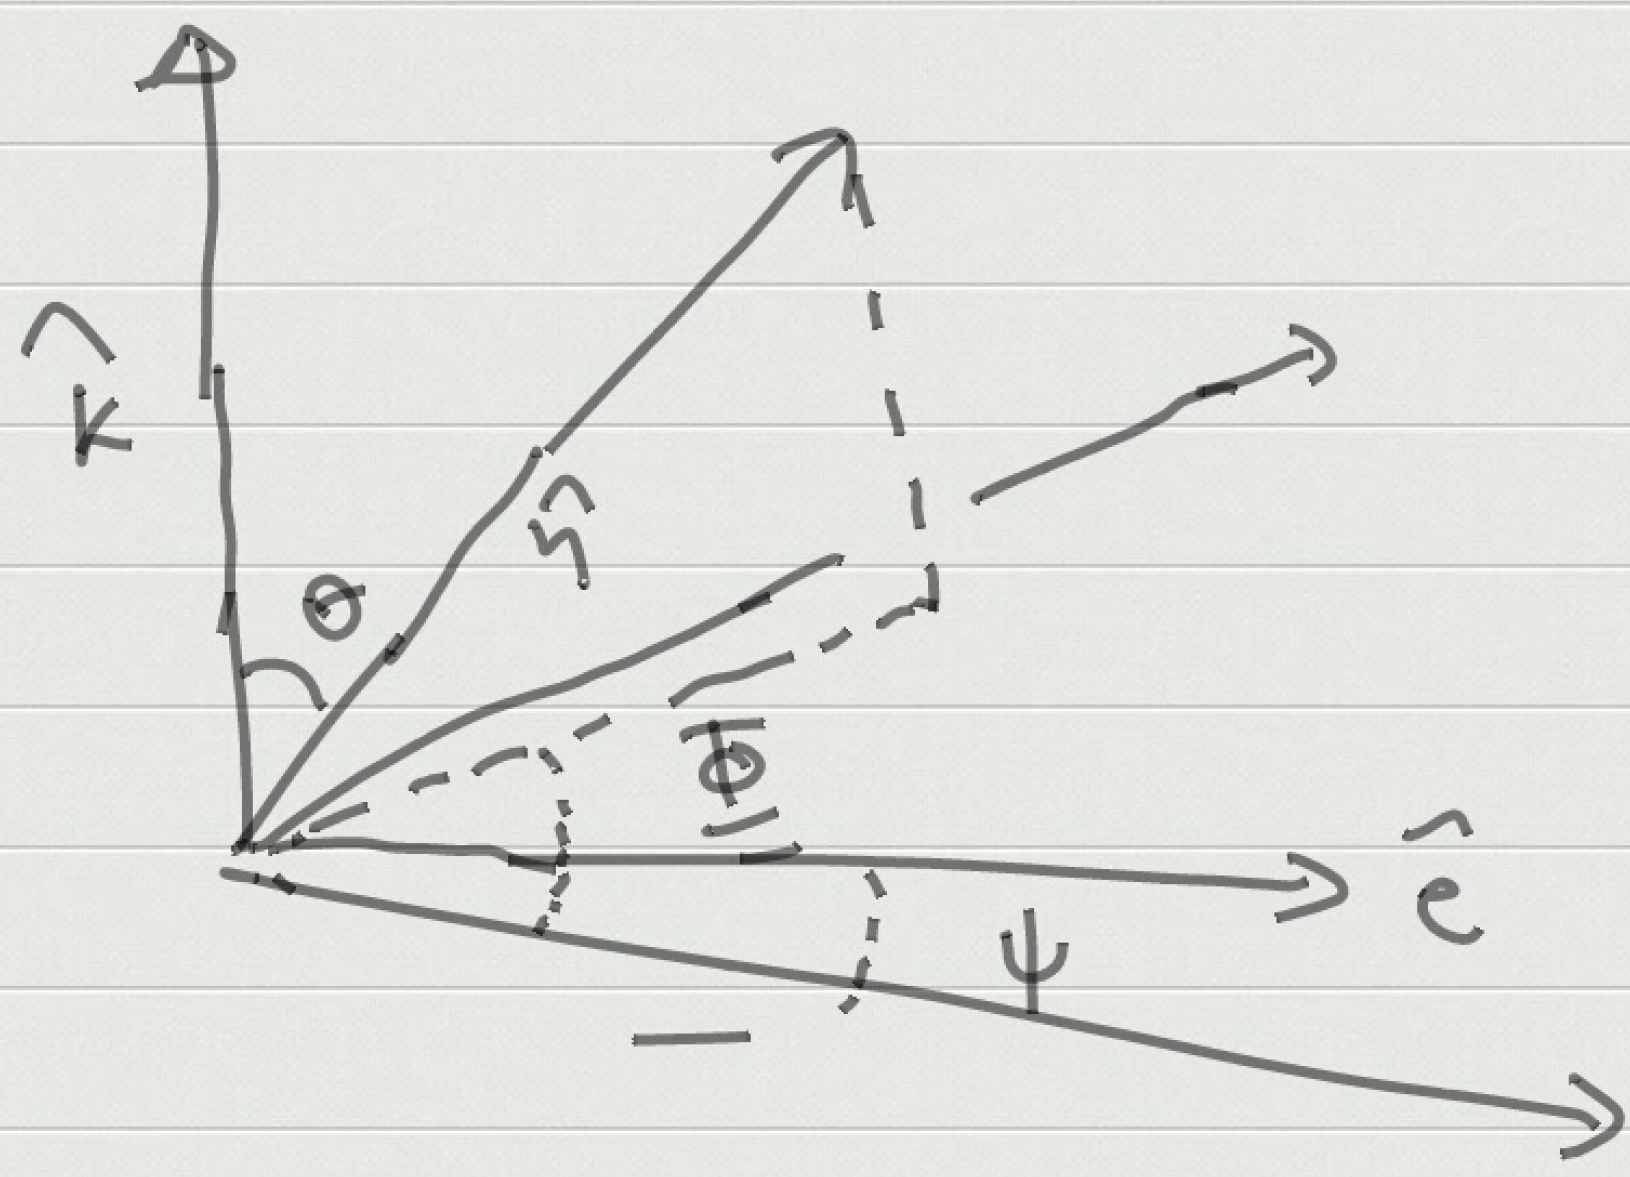
\includegraphics[width=0.9\textwidth]{Pictures/Scattering.png}
\end{minipage}

% \begin{figure}[h]
%     \centering
%     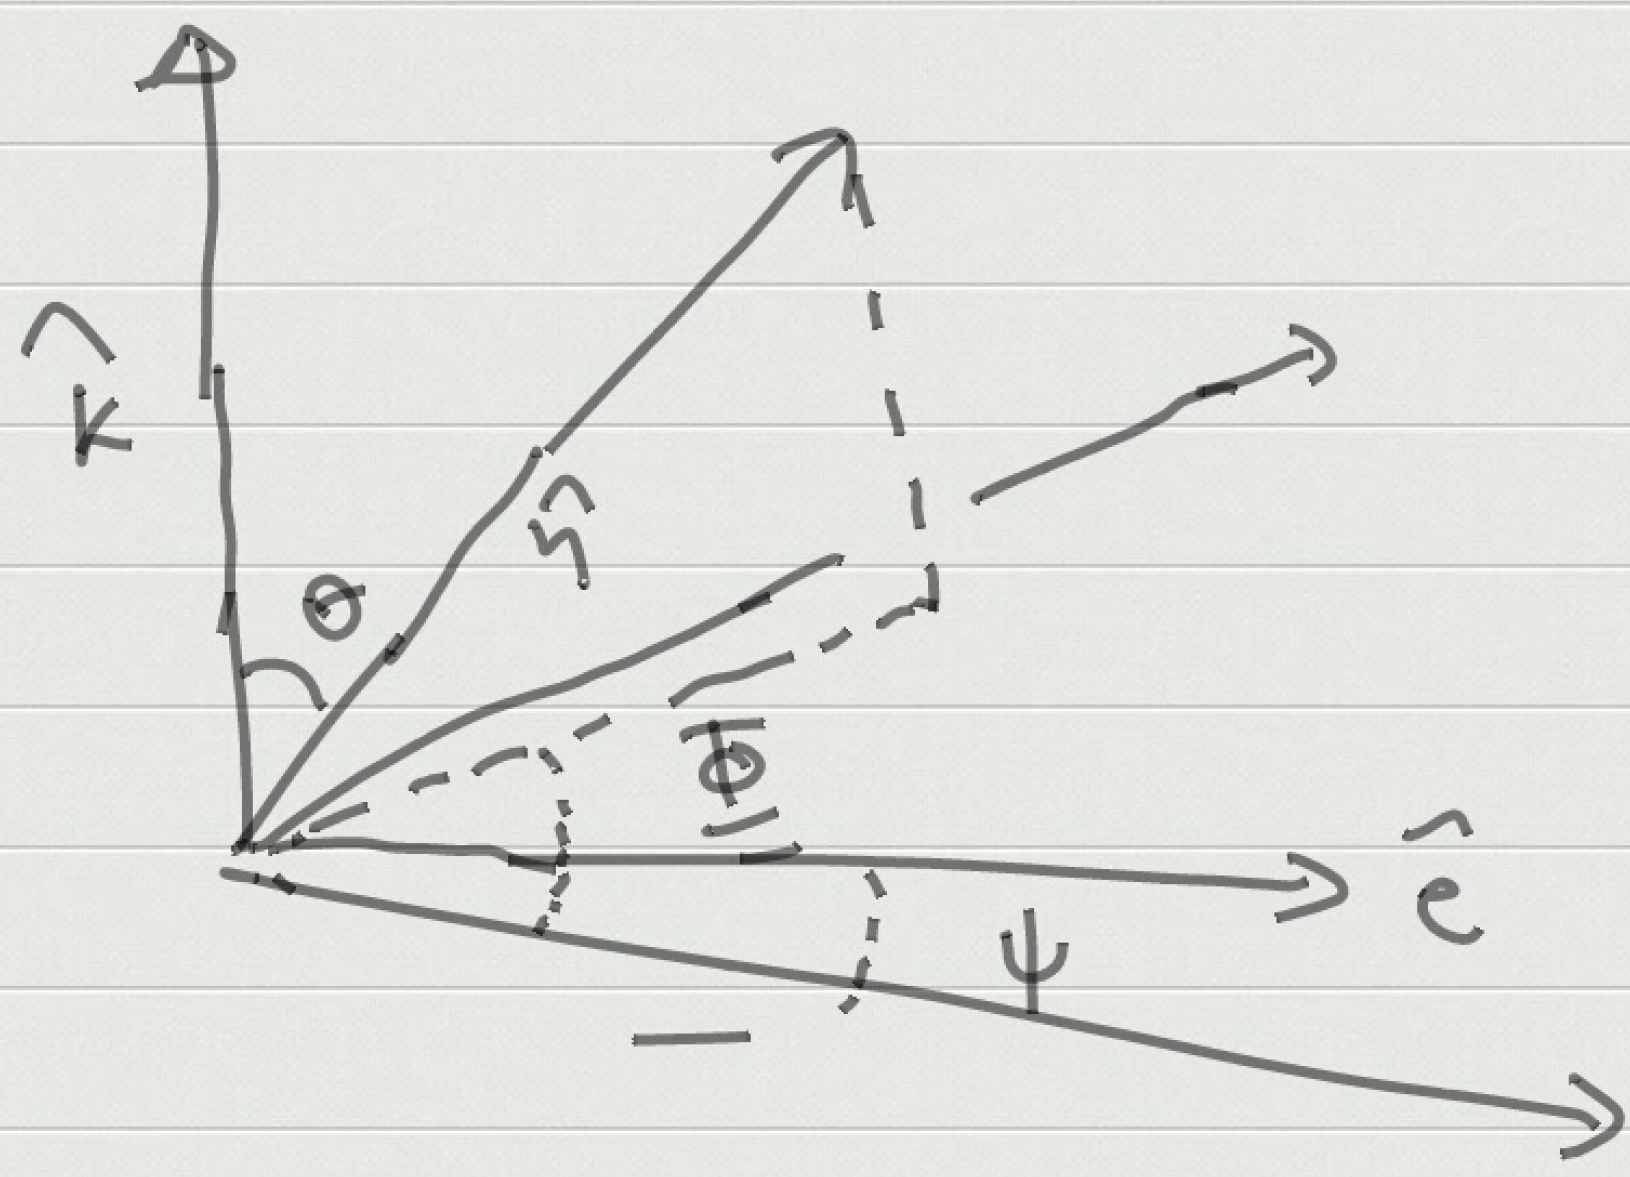
\includegraphics[width=0.2\textwidth]{Pictures/Scattering.png}
% \end{figure}

% The differential cross-section for unpolarised incoming photon beam:
% \begin{align*}
%     \frac{d \sigma}{d \Omega}
%     = \frac{q^4}{16 \pi^2 m^2} \frac{1 + \cos^2(\theta)}{2}
% \end{align*}
% The total cross-section is:
\begin{align*}
    \sigma = \int d \Omega \frac{d \sigma}{d \Omega}
    = \underbrace{\frac{q^4}{16 \pi^2 m^2}}_{\equiv r_q^2} \frac{8 \pi}{3}
    = \frac{8 \pi}{3} r_q^2
\end{align*}

We define the Thomson radius as:
\begin{align*}
    r_e \equiv \frac{e^2}{4 \pi \epsilonnull m_e c^2} \approx 2.8 \cdot 10^{-15} \mathrm{m}
\end{align*}
It can be understood as the effective radius of an electron if you assign to it
a spherical shape.

\subsection{Rayleigh scattering}

Now we examine the scattering of an electromagnetic wave on an electric charge
which is bound in an atom or molecule. The Equations of Motion and its
solution are:
\begin{align*}
    \frac{q E}{m} = \ddot{x} + \gamma \dot{x} + \omega_0^2 x
    \hspace{10pt} \Rightarrow \hspace{10pt}
    \vec{x} = \frac{\frac{q \vec{E}}{m}}{\omega_0^2 - \omega^2 + i \gamma \omega}
\end{align*}
The acceleration is then given as:
\begin{align*}
    \dot{\vec{v}} = \ddot{\vec{x}} = \frac{q \vec{E}}{m} \frac{-\omega^2}{\omega_0^2 - \omega^2 + i \gamma \omega}
    = \dot{\vec{v}}_{Thomson} \frac{-\omega^2}{\omega_0^2 - \omega^2 + i \gamma \omega}
\end{align*}
where $\dot{\vec{v}}_{Thomson} = \frac{q \vec{E}}{m}$. The crosssection is:
\begin{align*}
    \sigma = \sigma_{Thomson} \frac{\omega^4}{(\omega^2 - \omega_0^2)^2 + \gamma^2 \omega^2}
    \hspace{10pt} \text{with} \hspace{10pt}
    \sigma_{Thomson} \equiv \frac{8 \pi}{3} r_q^2
\end{align*}
For $\omega \ll \omega_0$ this process is known as Rayleigh scattering and the
crosssection becomes:
\begin{align*}
    \sigma_{Rayleigh} = \sigma_{Thomson} \frac{\omega^4}{\omega_0^4}
\end{align*}
